\chapter{Scientific Citations and Their Patterns}\label{Scientific Citations and Their Patterns}
"\textit{If I have seen further, it is by standing on the shoulders of giants}''. This famous quote by Sir Isaac Newton summarizes perfectly the
moral obligation of a scientist to acknowledge the contribution of previous works to their own. Newton was perfectly aware that his
groundbreaking discoveries would have been impossible without the fundamental work done by previous scientists, from Aristotle to Galileo 
and Kepler, covering  centuries, if not millennia of scientific and philosophical endeavours.
While the recognition of the work done by predecessors at the times of Newton was done primarily by mentioning the names in the text or in private correspondence (as was the quote mentioned before) as a form of intellectual courtesy,
in modern times it has taken the form in scientific journals of a moral obligation based on an agreed voluntary scheme and is considered as a fundamental part of good scientific practice,
while for patents it even has a legal side, with previous patents being cited in order to be able to clarify how the new patent differs substantially from previously similar ones.
 Furthermore, due to the limited space available in a text, along 
  with the gradual process that turns recent discoveries into common knowledge, the publications mentioned in the reference lists represent
  an extremely careful and precise process of selection of a very limited number of works among thousands, if not millions, of related works published
  in recent times.
  
  As the results in aging literature are slowly assimilated as basic findings, scientists move on to newer results as the basis of their works,
  thus implicitly determining when a groundbreaking result becomes obsolete, as more impelling results require their attention. Just like Newton chose to acknowledge
  Galileo for a few selected results, but ignoring to do to the same with Pythagoras and his extensively used theorem, a recent paper in Quantum Physics will hardly
  mention any of the works of Einstein's Annus Mirabilis even though they are the very foundation on which its work is based on, since their results are now
  accepted as being universally known and do not need to be individually addressed anymore. 
  
It is for these reasons that ever since the early times of scientometrics, a lot of attention has been given to the analysis of the individual performance of
a single publication in terms of citations. A simple citation count is a superficial yet quantitative evaluation of the success of a paper and is deemed sufficient by some
to be able to compare and rank publications as well as scientists. However, the aforementioned process of obsolesce in science adds a dimension which has been described as
an \textit{attention economy} \cite{klamer_attention_2002} in which authors are aware that they have a limited amount of time to gather attention (i.e. citations)
and therefore compete against each other in order to obtain the maximum attention available. 

Such complex aspects that lead to the selection of the cited material has been the source of even more interest into the citation patterns as well as statistics of citation counts across
disciplines, countries and through time. This chapter will go through the most relevant works that have investigated the citation patterns in science, looking at the basic properties in citation
habits and with a summary of the most interesting attempts at modeling mathematically the citation patterns of scientists.



\section{Citation distributions} \label{sec:Citation Distributions}
 
One of the earliest questions that scientometrics tried to answer already with de Solla's seminal paper \cite{deSollaPrice510} has been: \textit{What is the functional form of the distributions of citations?}.
In particular, since the average value of citations gathered is bound to be structurally low as its value is linked to the finite number of 
references available, the interest was in the tail of the distributions, that is what are the citation values and patterns for the 
few exceptional publications capable to gather a number of citations that span over multiple orders of magnitude.
De Solla claimed, based on his limited data, that the functional form was power law like, with the number of papers with $c$ citations behaving like $N(c) \propto c^{-\alpha}$, with an estimate of $\alpha \in [2.5,3.6]$. 

For a long time, no one looked further into the claim with only Laherrère and Sornette in 1998 \cite{refId1} suggesting a generic stretched exponential form for the citation distribution
of \textit{authors}. It was only in 1998 that S. Redner tackled the topic in a systematic way \cite{refId0}. It is important to notice that such analysis was possible to be carried out
mainly thanks to the availability of a properly catalogued data set of scientific publications. By using two large data sets (~700 thousand papers obtained from the Institute for Scientific Information (ISI) and ~24 thousand papers
from Physical Review D) combining for more than 7 million citations, the author was able, for the first time, to carry out a thorough computational statistical analysis of citation
distributions. The results offered an interesting and, to a certain extent, worrisome insight of the relative popularity of scientific publications: almost half of the papers
failed to gather any citation at all from publication date to the time of the study, with $80\%$ of the publications gathering 10 citations or less. Even though also de Solla noticed a huge amount of uncited papers,
Redner was able to confirm the pattern also for a larger and more significant data set. The author concluded that a final evaluation of the functional form of the citation distribution
cannot be thoroughly computed as the tail of the distribution has not reached its final state, as the highly cited papers are still gathering citations. He also pointed out how a few 
highly cited papers can affect the higher-order moments of the distributions, thus making the task even harder. However, Redner succeeded in gathering some indirect measurement through
a Zipf plot \cite{Zipf}, providing evidence of a power law behaviour with $\alpha \approx 3$, compatible with de Solla's findings. Furthermore, the author concluded with what can be considered
the \textit{cookbook} for future attempts at modeling the citation mechanism: a short memory (or Myopia) and the "rich get richer" kind of mechanism that was
introduced by de Solla himself in 1976 \cite{Price1976}. The latter would become a massive
topic starting from the following year, with Barab{\'a}si's work on scaling in random networks \cite{Barabasi509} which managed to mathematically justify the power law distribution of citations. 


Despite the case seeming to be settled, it was Redner himself in 2005 who challenged his own previous findings \cite{RednerStatistics}. In his later work, the author looked deeper in the 
PR data set, this time expanded to over 300 thousand papers from July 1893 through June 2003, suggesting that a log-normal distribution better describes the data.

A somewhat conclusive result in the discussion of the form of citation distributions came in 2008
with the work of Radicchi et al. \cite{Radicchi11112008} who found strong evidence for a lognormal distribution for the citation distribution of scientific publications and furthermore managed
to discover universal properties in the citation distribution across disciplines as different fields have. 
In their paper, the authors show how the citation distributions across fields, despite being apparently extremely different quantitatively,
can be mapped into a universal distribution if taking into account the statistical properties of each distribution. Differences
in citation counts across disciplines are a well known bias, the roots of which
lie in the different sizes of the fields or disciplines \cite{KING87} as well as in different conceptual meaning of the citation itself \cite{HURT19871}. In order to get rid of discipline dependent factors, the authors
introduced a new Relative Indicator (RI) $c_{f} = c/c_{0} $ for each paper, where $c$ is the number of citation the paper receives and $c_{0}$ is the average
number of citations received by articles published in its field in the same year and writing a functional form for the distribution of RI as $F(c_{f}) = \frac{1}{\sigma c_{f}\sqrt{2\pi}} e^{-[log(c_{f}) - \mu]^{2}/2\sigma^{2}}$, where 
$\sigma^{2} = -2\mu$ allows the expected value of $c_{f}$ to be 1, thus allowing to compare the distributions across disciplines. Radicchi et al. also reported that the collapsing behaviour persists also when distribution from different years are compared, therefore suggesting that the functional form mentioned before
is a \textit{universal} curve, thus allowing to compare citation counts across fields and times in a fair way. 

Field dependent patterns are also known to cause
to disproportionate citation counts, even though they can be quantified and corrected for. This can be achieved by
"imposing" a mapping between cumulative distributions of citations for papers published in a single category (i.e. subfields or fields) to the aggregated cumulative citation distribution  \cite{10.1371/journal.pone.0033833}. For each field
is therefore possible to assign to each citation count $c'$ in the field cumulative distribution $P_{f}(\geq c')$ to the corresponding value $c$ in the aggregated cumulative distribution
($P(\geq c)$) such that $P_{f}(\geq c') = P(\geq c)$. The relation between the two values for different fields is show in Fig. \ref{fig:radicchi_citations} as a quantile-quantile plot, in which
it can be seen that the two citation measures are connected by a power law relation, therefore suggesting that the main difference between the citation distributions across
fields lies only in a difference in each field's scaling factor.

\begin{figure}[h!]
\centering
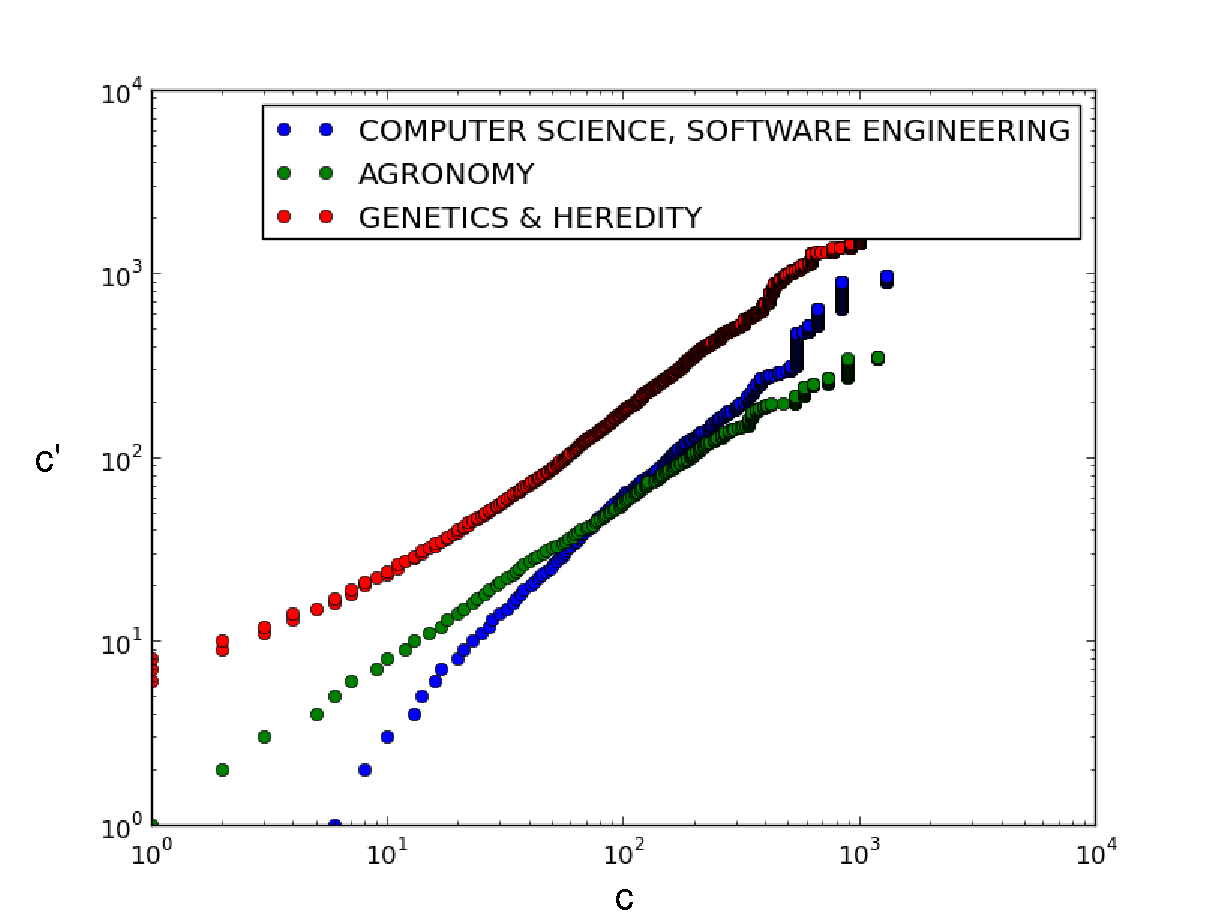
\includegraphics[width=.8\textwidth]{radicchi.pdf}%
\caption{$c'$ vs $c$ adapted from \cite{10.1371/journal.pone.0033833} and reproduced with our data set. We can see that the scaling follows the relation: $c' = ac^{\alpha}$ where
a is a pre-factor and $\alpha$ is a field dependent scaling factor.}
\label{fig:radicchi_citations}
\end{figure}

\pagebreak
\newpage


\section{Biases in citations}

In 2005 Hajra et al. were \cite{Hajra200544} were among the first ones to suggest a temporal aspect in citation dynamics and decided to look at the impact that age has on citations. By looking at the citation dynamic of a 
set of papers, they found a critical time $t_{c}$ of 10 years, after which the rate at which citations are gathered drop significantly, indicating that papers have approximately a \textit{lifespan} of 10 years. In another paper in the 
following year \cite{Hajra2006575}, the authors suggest that the \textit{rich get richer} mechanism might require to be connected with an aging of the publications in order to take into account the obsolesce
of scientific publications. In Publication II we confirmed this property, showing that the typical life cycle of a paper is becoming shorter in time. Fig.\ref{fig:peak_decay} shows the evolution of the time to reach the 
peak of citations for top papers in a selected number of fields.
\begin{figure}[htpb!]
\centering \large
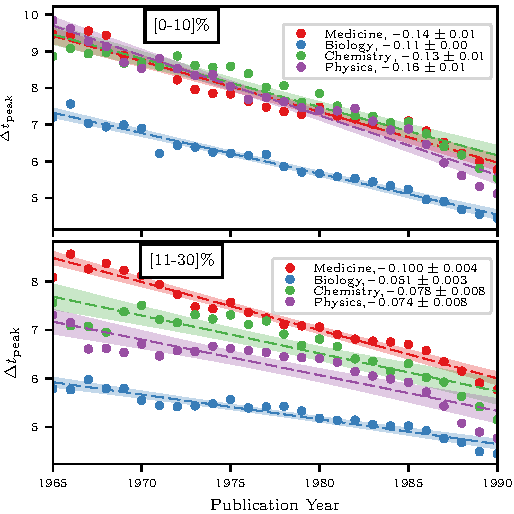
\includegraphics[width=.8\linewidth]{Figures/Fields_Peak_stats_Mean.pdf}
\caption{ Time evolution of the mean values of time to peak $\Delta t_{{peak}}$ for top 10$\%$ (top) and [11-30]$\%$ percentiles (bottom) of our ISI dataset. $\Delta t_{\mathrm{peak}}$ 
represents the time elapsed between the publication of a paper and the year in which it reached its maximum yearly citation count.
The mean value $\langle \Delta t_{\mathrm{peak}} \rangle$ decreases linearly in time. The linear fit, $95\%$ confidence interval and the slopes of the linear fits are also shown. Figure adapted from Publication II.}

\label{fig:peak_decay}
\end{figure}

While the average suggests that papers are being forgotten within a limited period of time, other works have been looking at the opposite phenomenon, the one of \textit{sleeping beauties}, i.e.
scientific papers that remained almost citationless for a long period of time only to become suddenly highly influential and cited \cite{Ke16062015}. The authors designed a Beauty coefficient defined as
$B = \sum_{t = 0}^{t_{m}} \frac{\frac{c_{t_{m}}- c_{0}}{t_{m}} * t + c_{0} - c_{t}}{max \{1,c_{t}\}}$ , where $ c_{t_{m}}$ is the maximum number of yearly citations gathered at time $t_{m} \in [0, T]$ and $T$ is the time 
at which the coefficient is measured. The coefficient 
therefore quantifies how "unexpected" the citation history of a paper is, with $B=1$ being the coefficient for a paper that grows linearly at a steady rate. One of the most interesting results of the study is that
sleeping beauties, albeit appearing to be extreme cases, are impossible to distinguish from the core of all papers, as there is no minimum $B^{*}$ value that allows to define a sleeping beauty as such. While most 
values of $B$ are shown to be low, the authors conclude that it is an intrinsic property of scientific output to have a vast heterogeneity in the times at which recognition takes place. These results
make particular sense for field such as Physics or Chemistry, where the theoretical and experimental sides of the same field are not always synchronized. 

One of the most evident examples of this asynchronism is the recent experimental discovery of the Higgs
boson, the existence of which was originally proposed in the 60s \cite{PhysRevLett.13.508} but was confirmed only in 2012 thanks to the development of the LHC at CERN in Geneva \cite{Aad20121}. The search of the boson was lagging so much behind that still 10 years after the 
theoretical breakthrough the hopes of a search for the Boson seemed remote despite phenomenological studies regarding its discovery had already started \cite{1201.6045}, as one of these studies points out \cite{ELLIS1976292} :

\textit{“We should perhaps finish our paper with an apology and a caution.
We apologize to experimentalists for having no idea what is the mass of the Higgs
boson, ..., and for not being sure of its couplings to other particles, except that they are
probably all very small. For these reasons, we do not want to encourage big experimental
searches for the Higgs boson, but we do feel that people doing experiments vulnerable to the
Higgs boson should know how it may turn up.”} 

The temporal aspect of recognition of older theoretical breakthroughs was a central source of inspiration for Publication I. In the paper we looked at the time lag between the publication of Nobel discoveries and 
the conferment of the prize, finding that it has been increasing at a very high rate, to the point where the original authors might pass away before seeing their discoveries empirically confirmed as shown
in Fig.\ref{fig:nobel_delay}. These findings
led us to conjecture that we are potentially in presence of two opposite scenarios: either the frequency of groundbreaking discoveries is
decreasing or, conversely, it could be that too many significant results are being published and that older discoveries are being awarded in order not to forget worthy winners.

 \begin{figure}[h]
\centering
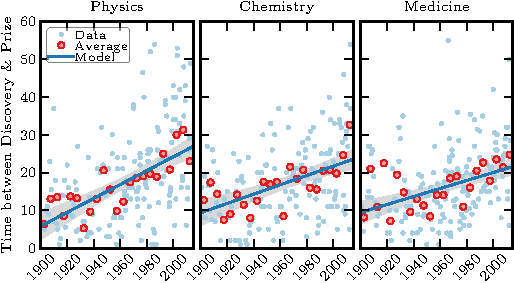
\includegraphics[width=.8\textwidth]{combined_PrizeSinceDiscovery.pdf}%
\caption{Time lag between discovery and Nobel prize vs year in which the prize was awarded for Physics, Chemistry and Medicine, created with data from Publication I. For each Nobel prize we searched bibliographic material on the author in order to
identify one or more publications that could be directly associated to the awarding of the Nobel prize. The blue dots represent individual discoveries, while the red dots
are a 5 year average over all awards in the bin. We can see a clear increase in average lag as well as the presence in more recent year of extremely high values (lag $\approx 50$ years). Figure adapted from Publication I.}
\label{fig:nobel_delay}
\end{figure}


Furthermore, one author might not be even aware of certain scientific works if he has not had the chance to read them or to search them
efficiently. Even though the limitations of access to scientific knowledge might have become less relevant in modern times thanks to the rise of the Internet era and immediate access to online catalogues, at the same time the possibility
to browse more recent material has consequently introduced a change in the way authors update their knowledge. The effects on the scientific community were rapid, as in 2003 already De Groote et al. \cite{pmid12883574}
showed through a survey that general users of scientific material prefer digital copies to printed ones. 
The constant need for immediate access to recent scientific knowledge has become such a relevant aspect of science itself that it has led to suggesting a ranking of journals in terms of the speed at which their publications 
complete their cycle \cite{JournalRankingSchemes}. 

An interesting study in the impact of online available material on citation patterns came in 2008 when Evans \cite{Evans395} studied the 
effect of online availability
of journal issues within the citation patterns of the journals and reported that the rise of online available publications shifted the citation patterns. The results showed that the more journals started to appear online, the more the reference list tended to be pointing at more recent discoveries and caused a \textit{concentration}
of citations towards fewer articles and fewer journals, an effect the authors claim is caused by hyperlinking, i.e. the search of further bibliographic material from the reference lists of papers previously read.

Recently however the claim has been challenged by Verstak et al. \cite{DBLP:journals/corr/VerstakASHILS14} as well as by Pan et al. \cite{DBLP:journals/corr/PanPPF16}.
Verstak et al. used Google Scholar Data to analyze all publications available between 1990 and 2013. The authors calculated the fraction of references in these papers pointing at least 10 years before the year of publication
for each paper and found that such fraction is actually \textit{increasing} in time. Furthermore, they noticed that the value of the change over the second half of the period 
studied was much larger than in the first,
with the former matching the period in which digitalization has took place (2001-2013). The authors therefore concluded that the accessibility of older material has allowed scientists to cite the most suited paper that they were
able to find, regardless of the time at which it was published. The latter paper by Pan et al. instead devised a model to test Evans' hypothesis which builds a citation network in which papers choose whom to cite 
both by "browsing" (i.e. by searching previous publications freely) and by a \textit{redirection} link-formation mechanism in which knowledge is found
by following the reference list of a source article previously browsed. By controlling the rate at which these two processes take place the authors
simulated a spark in the redirection mechanism, representing the availability of online journals. The model showed that the redirection mechanism had very little impact on the average age of citations, while the growth of the system
appeared to have a much more significant role. 

The constant increase in scientific works might limit the ability to physically and mentally keep track of all relevant publications being published. This might be among one of the
greatest limiting factors in citation patterns, as it has been reported 
 \cite{doi:10.1108/00012530910932267} that scientists read more papers, yet
dedicating less time on average to each one. 
The temporal dimension of the 
citation selection process has been the key source of inspiration for Publication II, where we suggest that the increasing number of publications causes a constant shift in focus towards more recent papers, therefore
shortening the citation life cycle of papers both in terms of time to reach their peak in popularity, as well as in terms of time needed to stop gathering significant citations after the peak. Fig. \ref{fig:attention_decay} shows the main results
of the analysis.

\begin{figure}[htpb!]
\centering \large
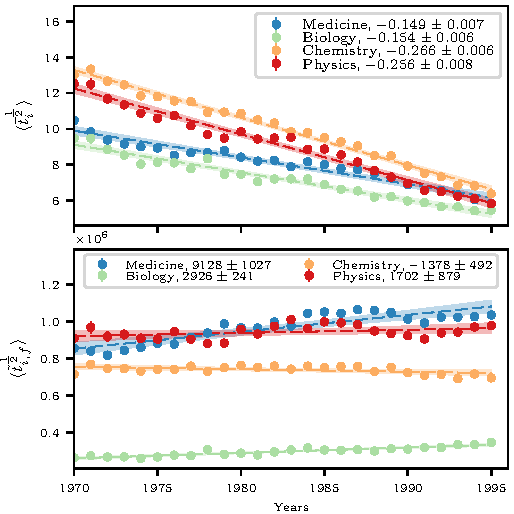
\includegraphics[width=0.8\linewidth]{Figures/LastAbove_0_10_5_finalPaper.pdf}
\caption{ The evolution of the half life of papers after the peak $\langle t_{i}^{\frac{1}{2}} \rangle$ in terms of absolute time (top) and $\langle \widetilde{t}_{i,f}^{\frac{1}{2}} \rangle$  in terms of the number of publications (bottom)
for the four different fields and for the top 10$\%$ percentile. For each paper we calculated the time
required for the publication to drop below half of the number of citations gathered in its peak year. We then proceeded
to average the values for papers published in the same field and peaking in the same year. The half life has been calculated both in terms of number of years and in terms of number
of paper published within the field in the same time interval. 
The linear fit, $95\%$ confidence interval and the slopes of the linear fits are also shown. The dashed line represents the linear fit. Despite its noisy behavior, the
renormalized half-life shows a relatively stable trend throughout the years, possibly with the only exception of Medicine and
Biology, which show a slightly rising pattern for recent time. Figure adapted from Publication II.}
\label{fig:attention_decay}
\end{figure}

Another aspect that influences citation choices is one that looks at the role that the individual authors play. Science is not only a philosophical endeavour, but also a social system where scientists personally interact
and collaborate and therefore are more exposed to works coming from a familiar set of collaborators or, in general, people working in the same area of research. Early research in fact showed that \cite{ASI:ASI10369} intellectual ties based on shared content surpass friendship as a predictor of reciprocal citation. Similarly, Persson et al. \cite{Persson2004} showed in 2004 that collaboration leads to a positive effects in the success of a paper, in particular if
the authors come from different countries.
This can be seen as a success linked to the possibility of the same work to be pushed forward at twice (or more) the same rate as a single author paper in different
"market pools" of customers, i.e. potential citers.  Furthermore, in 2004 Gl{\"a}nzel et al. reported that multi-authorship increases the chances of self citation \cite{Glanzel2004}, with the number of authors not being a factor though. However, the authors point out that
the most dominating contribution of multi authorship is the increase in foreign citations, thus showing the social contribution of a multi author paper in terms of geographical advantage. 

The topic of self-citations is
a highly debated one in a world where citation metrics are used as tools to quantify careers and quality of research. The same author showed in another paper in the same year that  self citations are an \textit{"Essential part
 of scientific communication"} \cite{Wolfgang2004}, but that its contribution plays a higher role in the immediate times after publications. This result, linked with empirical evidence of self-citation being correlated with publishing on average in journals with
relatively low impact shows that this trend might be linked to the need of a "push" in fame, hoping for success to accumulate from there. However, while self-citation does appear to have an impact on citation counts,
it is not clear whether the correlation is linked to a matter of \textit{visibility}, i.e. trying to put forward one's results as a "bandwagon" effect, or rather a matter of \textit{quality}, as one author
mentions its own best works as a basis for future ones \cite{Fowler2007}. More recent results confirm  \cite{10.1371/journal.pone.0033339} that the trend is still significant, yet retaining different patterns in different fields, due to the 
possibility of certain fields to have many groups working on independent topics, thus focusing the selection of cited material from a smaller subset of works. The authors also report that a higher propensity in inter-author-citations
leads to a higher chance of inter-citations of the second order, with collaborators of collaborators being more likely to be cited. 

Authors might also influence their own career retroactively as shown by Mazloumian et al. \cite{10.1371/journal.pone.0018975}. The authors
found that groundbreaking results by an author have a positive impact on their own previous literature, therefore creating a status of authority for the author even though the earlier works
might not be necessarily related to the successful recent ones both in terms of topic and intrinsic scientific quality. The role of prestige in science is so critical that it has been
suggested to also be a bias within the peer review mechanism \cite{ASI:ASI22784}. This psychosociological mechanism that enhances the career of already successful scientists
based on their academic reputation is often called \textit{Matthew Effect} and its impact on science has been discussed since the 60's \cite{MatthewEffect}. In general, a citation bias towards successful papers (preferential
attachment) and one towards successful authors (Matthew Effect) shows that the citation mechanisms are not only based on scientific necessity, but are also based on individual and collective aspects that emerge from the
human interaction between scientists. Finally, it is worth to mention that there are plenty of other factors that influence citations, such as journal-dependent factors, field-dependent factors
and technical ones \cite{doi:10.1108/00220410810844150}, which will not be analyzed for the sake of brevity.






\section{Modeling}

The previous section showed how many factors and biases play a role in the mechanisms underlying the decision of which papers will appear on a reference list, with empirical results showing heterogeneous results within
the same field of analysis. It is therefore not surprising that the pursuit for a mathematical model that could correctly reproduce the properties of citation mechanism has been a challenging one, which scientists however
were eager to undertake in order to shed more lights on the way science itself works, focusing in particular on the temporal aspect of the models.

The earliest and most successful attempts at modeling citation dynamics lie in the \textit{rich get richer} or, technically speaking, \textit{preferential attachment} mentioned in the previous sections . Despite the original idea was already
formulated in de Solla's work \cite{deSollaPrice510}, it was Barab{\'a}si in 1999 who was able to mathematically describe it exhaustively \cite{Barabasi509}.
In his work, Barabasi suggests a model (PAM) in which the probability (or attachment rate)
$A$ of a paper  of receiving another citation from a new paper is directly proportional to the number of citations $c$ citations previously collected: $A (c) \propto c$.
This mechanism is able to explain
the citation distribution both from a qualitative point of view (its fat tailed behaviour) as well as numerically, confirming an expected value extremely close to 3 for $\alpha$. 
Interestingly, the model was applied to a vast amount of complex systems, with particular success in biology \cite{Barabasi2004,Jeong2000}, of which citation dynamics represent one of the examples.

A confirmation of the validity of the preferential attachment mechanism came in 2005 with Redner \cite{RednerStatistics}, who reported that the attachment rate is indeed linear, leading to a double paradox: the linear attachment rate 
shown by the data should lead to a power law distribution for citations, while data shows that the form is log-normal, which in turn would require an attachment rate of the form
$A_{c} = \frac{c}{1 + a \ln(c)}$ with $a > 0$. Despite confirming empirically the validity of a linear form of preferential attachment, Redner suggests that the underlying assumptions
behind the preferential attachment model, when applied to science, might be not completely realistic, as the model implies a full knowledge of all the corpus of existing papers, a
challenge which has its limitations both in terms of accessibility as well as in terms of memory. 


As we saw in the previous section however, it is fundamental to introduce the  question of time dependence within the modeling framework. While theoretical works tried to tackle the topic from a purely mathematical standpoint \cite{Amaral2000,PhysRevE.68.056121}, it 
was Hajra et al. \cite{Hajra200544} in 2004 who applied it with success to the modeling of citations. 
The authors followed the previous theoretical works and formulated a functional form for the attachment rate of 
$\Pi(c,t) = C(c)T(t)$, where $C(c)$ and $T(t)$ are generic functions and where the attachment rate is assumed to be separable. The authors then tried to identify the functional form for the temporal aspect that would best fit the data through the analysis of the distribution of citation ages $Q(t)$, i.e. the raw distribution
of the fraction of citations with age $t$. In order to do so, the authors took
into consideration the stochastic nature of the rate at which new citations appear, i.e. the rate at which new papers are published. Therefore by empirically estimating from their data sets a publication rate
of $n(t) = a(1 - e^{-bt})$ they were able to renormalize the distribution and obtain a functional form of $T(t) = \frac{Q(t)}{n(t)}$. Comparing the model with the collected data, the authors identified
two  distinct regimes of power-law decay of the distribution: $T(t)\sim t^{-\alpha_{1}}$ for  $0<t<tc$  and $T(t) \sim t^{-\alpha_{2}} $ for $t>t_{c}$ where $t_{c} \sim 10$ is the expected lifespan of a paper mentioned earlier.

In Publication II we proposed a model for the process of gathering new citations as a \textit{counting process}. In this ultradiffusive framework, the arrival of a new citation is hypothesized to be  correlated to an earlier event or a combination of events.
Therefore, 
ultradiffusion
proposes that the pattern of events emerges as a consequence of an underlying hierarchy of states, in which a more recent event is more likely to affect the future ones. Our results, that show an exponential fall
in citation after reaching the peak, which is slowly transitioning into a power law pattern is coherent with the hypothesis of an ultradiffusive process driving the attraction of new citations.
This framework is known to be 
able to explain the evolution of the response to new pieces of information online \cite{ghosh_information_2013}, allowing us to draw a comparison between the way in which attention is dedicated to new publications and the way
readers react to news. 


A further improvement on the PAM came in 2008 with a work by Wang et al. \cite{Wang20084692}. Their model proposes to not separate globally the dependence of the attachment rate on the two variables, considering the aging
process to be related not to the whole paper, but to the citations themselves. The logic behind this idea is that a paper that has received a lot of attention lately (a sleeping beauty for example) will be more likely
to gather new citations if compared to a paper published in the same year, with a similar citation count, but having failed to receive citations recently. Therefore, the authors express the rate as $\Pi(c,t)  \propto \sum_{t} c_{i}f(t_{i}) \propto  \sum_{t} c_{i}exp(-\lambda t_{i}) $,
where $k_{i}$ are the citations gathered in year $t_{i}$ and the exponential form for the weights is taken from fitting data, a scheme they call Gradually-vanishing Memory Preferential Attachment Mechanism (GMPAM). 
While the empirical data shows a good accordance the model, the authors admit that the model is somewhat excessively complicated, as it requires to calculate weights for decades of citation data coming from
  different citation pools (field and geographical biases above all) that require to fine tune the value of $\lambda$ case by case. The authors therefore proceed to simplify the model, by observing that the most 
  significant temporal contribution to the attachment rate comes from the most recent number of citations, i.e. the number of citations gathered in the last year. The temporal aspect therefore it's taken to be
  as a \textit{memory effect}, that makes the older citations be "forgotten", giving priority to papers that are riding a popularity wave. The updated model, called Short-term Memory Preferential Attachment Mechanism (SMPAM) thus expresses
  the attachment rate as $\Pi(c,t) \propto c_{t-1}$. 

Similarly, other authors have decided to focus the modeling part only to reproduce certain aspects of the citation dynamics with still a focus on the temporal aspect.
In 2001 Burrel was able to confirm that a stochastic process that assigns citations to publications 
based a non-homogeneous Poisson process \cite{Burrel2001} is bound to produce articles that will remain uncited. In 2009 Wallace et al \cite{Wallace2009296} tried to model the citation distribution of publications by separating the citation curve in different areas, developping in particular a model able to quantify the impact
of uncited papers in the citation distribution. The authors hypothesized that the probability for a certain paper to receive an initial citation depends only on the number of articles $N_{A}$ published in the same year
 and the number of references $N_{R}$ available in the following year, with citations being given randomly through a Poissonian distribution, given the size of the two variables. The authors then limit the 
 probability of citing an uncited paper to the field-dependent rate at which uncited papers are cited for the first time. It therefore follows that the pool of available references is reduced to $\beta_{I}N_{R}$, where $\beta_{I} \in [0,1]$ is extracted
 from the data, and that the probability for a single paper to fail to receive any citations is:
$\Phi_{I} = e^{-\beta_{I} (N_{R}/N_{A}) }$. 

 
In 2009, Newman \cite{0295-5075-86-6-68001} published a study which added to the temporal aging process the aspect of novelty, the so called
\textit{first mover effect}.  The idea behind the work is that science is based on the production of new results and therefore there is an intrinsic advantage in the being the first ones to publish a new result in a field,
since future works are bound to cite the paper introducing the novelty. In his paper, the author works with previous models based on preferential attachment to build a new one where on average newly published papers cite
$m$ earlier papers, chosen proportionally to the number of citations $k$ they already have, plus a variable $r$ needed to ensure
that uncited papers still have a nonzero probability of being cited. From this model one can calculate the average number of citations $\gamma$ a paper is expect to receive at time $t$ as: $\gamma(t) = r(t^{-1/(\alpha - 1)} -1)$, where $\alpha =  2 + r/m$.
Therefore, it follows that older papers (i.e. $t \rightarrow 0$) should on average receive far more citations than
those published later, even taking into consideration the the fact that later
papers have less time to gain citations.

These results are somewhat in contrast with the previous discussion regarding obsolescence and the time span of papers. 
However, Newman himself points out that the first mover advantage is limited to scenarios in which the results
are not part of a  larger, already established field, but rather represent the emergence of new subfields or fields altogether, as their analysis of citation data in fact seems to confirm. 


In 2011 Eom and Fortunato  \cite{10.1371/journal.pone.0024926} published a paper in which the aspect of the \textit{burstiness} in science is tackled. Burstiness is a sudden and intermittent modification of the 
frequency of an event,  which has been known to play a fundamental role in many human dynamics \cite{0295-5075-81-4-48002,PhysRevE.83.025102}. In this context, burstiness represents all sorts of inhomogeneous fluctuations that
lead to a sudden and unexpected rise in the citation count of a paper, which can be expressed as $ \Delta c/c = [c(t+\delta t)^{i}_{in} - c(t)^{i}_{in}]/c(t)^{i}_{in}] $, where $c(t)^{i}_{in}$ is the number of incoming citations
a paper received at time $t$ measured in years. This rate therefore measures the relative change in citations during the period of time $\delta t$, compared to the history of citations of the paper. Data shows that the distribution
of these rates is fat tailed for $\delta t = 1$, showing therefore that it is possible for a paper to suddenly receive orders of magnitude of citations more than they ever did, especially during its early years. Similarly to what happens to sleeping beauties, burstiness shows that there can be stochastic driving forces that cannot be ignored and that a linear model with no memory
or time dependence cannot grasp. The authors therefore propose a model still based on the preferential attachment model, where however each papers has an intrinsic \textit{attractiveness} that depends on time. The result is a model in which a new paper $i$
cites $m$ new papers, with the probability of a certain paper $j$ to be cited described as : $\Pi(i \rightarrow j ,t) \propto [ c^{j} + A_{j}(t)] $. For the form
of the attractiveness the authors assume an exponential decay $A(t) = A_{0} exp^{-(t-t_{0})/\tau}$, where $\tau$ is the time scale at which the temporal dimension plays a role, with initial attractiveness taken from a power law in order 
to best fit the data. Once again, we have a model
where a linear preferential attachment is mixed with a temporal dimension, which in this case takes into account random fluctuations of the citation history of the paper that
alter the expected individual citation trajectories. Attractiveness can be seen as proxy of an intrinsic \textit{quality} of the paper, which is explicitly separated by the success of a paper in terms
of citation. The model therefore suggests that citations do not represent the absolute measure of the quality of the paper, but that rather they are a probable (but not guaranteed) consequence
of papers of high quality (attractiveness). However, with citations and preferential attachment still being a fundamental driving force of the citation market, an initial failure to gather an initial minimum number
of citations might be sufficient to prevent a high quality paper from rising to notoriety. 

In 2015 Wang et al. \cite{Wang127}, including the original proponent of the Preferential Attachment Model
Barab{\'a}si tried to further expand the concept of separating the driving force of citation and the one of fitness of the individual paper, by proposing an attachment rate of the form:
$\Phi_{i}(t) \propto \eta_{i}P_{i}(t,\mu_{i},\sigma_{i})c_{i} $, where $\eta$ is the fitness of the individual paper and $P_{i}(t,\mu_{i},\sigma_{i})$ represents the aging process of the ideas introduced by the paper. The separation of fitness
from aging (i.e. it's not the fitness that decays, but rather the \textit{novelty}) comes at a cost, as the authors needed to introduce two new parameters, represented by the immediacy $\eta$ of a paper and
its longevity $\sigma$ which determine the time at which a paper reaches its peak of notoriety and how long its notoriety will last respectively. The model is therefore able
to predict the future citation trajectory of a paper, given a previous window of time during which its intrinsic parameters can somehow reveal themselves and be quantified
through a least square fit method. Furthermore, the authors managed to quantify the importance of the individual contributions within the attachment rate formula, finding that
the dependence on the number of citations (i.e. the classical model) is triggered only when a paper crosses the threshold of seven citations, below which it's the paper attractiveness that 
dominates.


